\documentclass[../Report.tex]{subfiles}


\begin{document}


\chapter{Einführung}
\label{chap:einfuehrung}
Mit den Barrier Bucket (BB) RF Systemen können am neu entstehenden Synchrotron SIS100 oder im Experimentier Speicherring (ESR) am GSI Helmholtzzentrum viele longitudinale Manipulationen am Teilchenstrahl vor genommen werden. Der dazu benutzte Spannungspuls hat die Form wie in \figref{BB_req} dargestellt. Wenn die Wiederholfrequenz des Spannungspulses gleich der Umlauffrequenz ist, so wird im Phasenraum eine stationäre Potential Barriere erstellt. Wenn die Wiederholfrequenz nicht gleich der Umlauffrequenz ist verschiebt sich die Potential Barriere im Phasenraum und es entstehen Bunches mit unterschiedlicher Länge. \\ Der Anspruch an diese Systeme liegt darin eine hohe Qualität des Impulses am Gap der Kavität zu erzeugen. Um sogenannte Microbunches zu verhindern müssen die Nachschwinger nach dem Einzelsinus kleiner als 2,5\% von $\hat{U}_{BB}$ sein. 
\begin{figure}[h!]
  \centering
    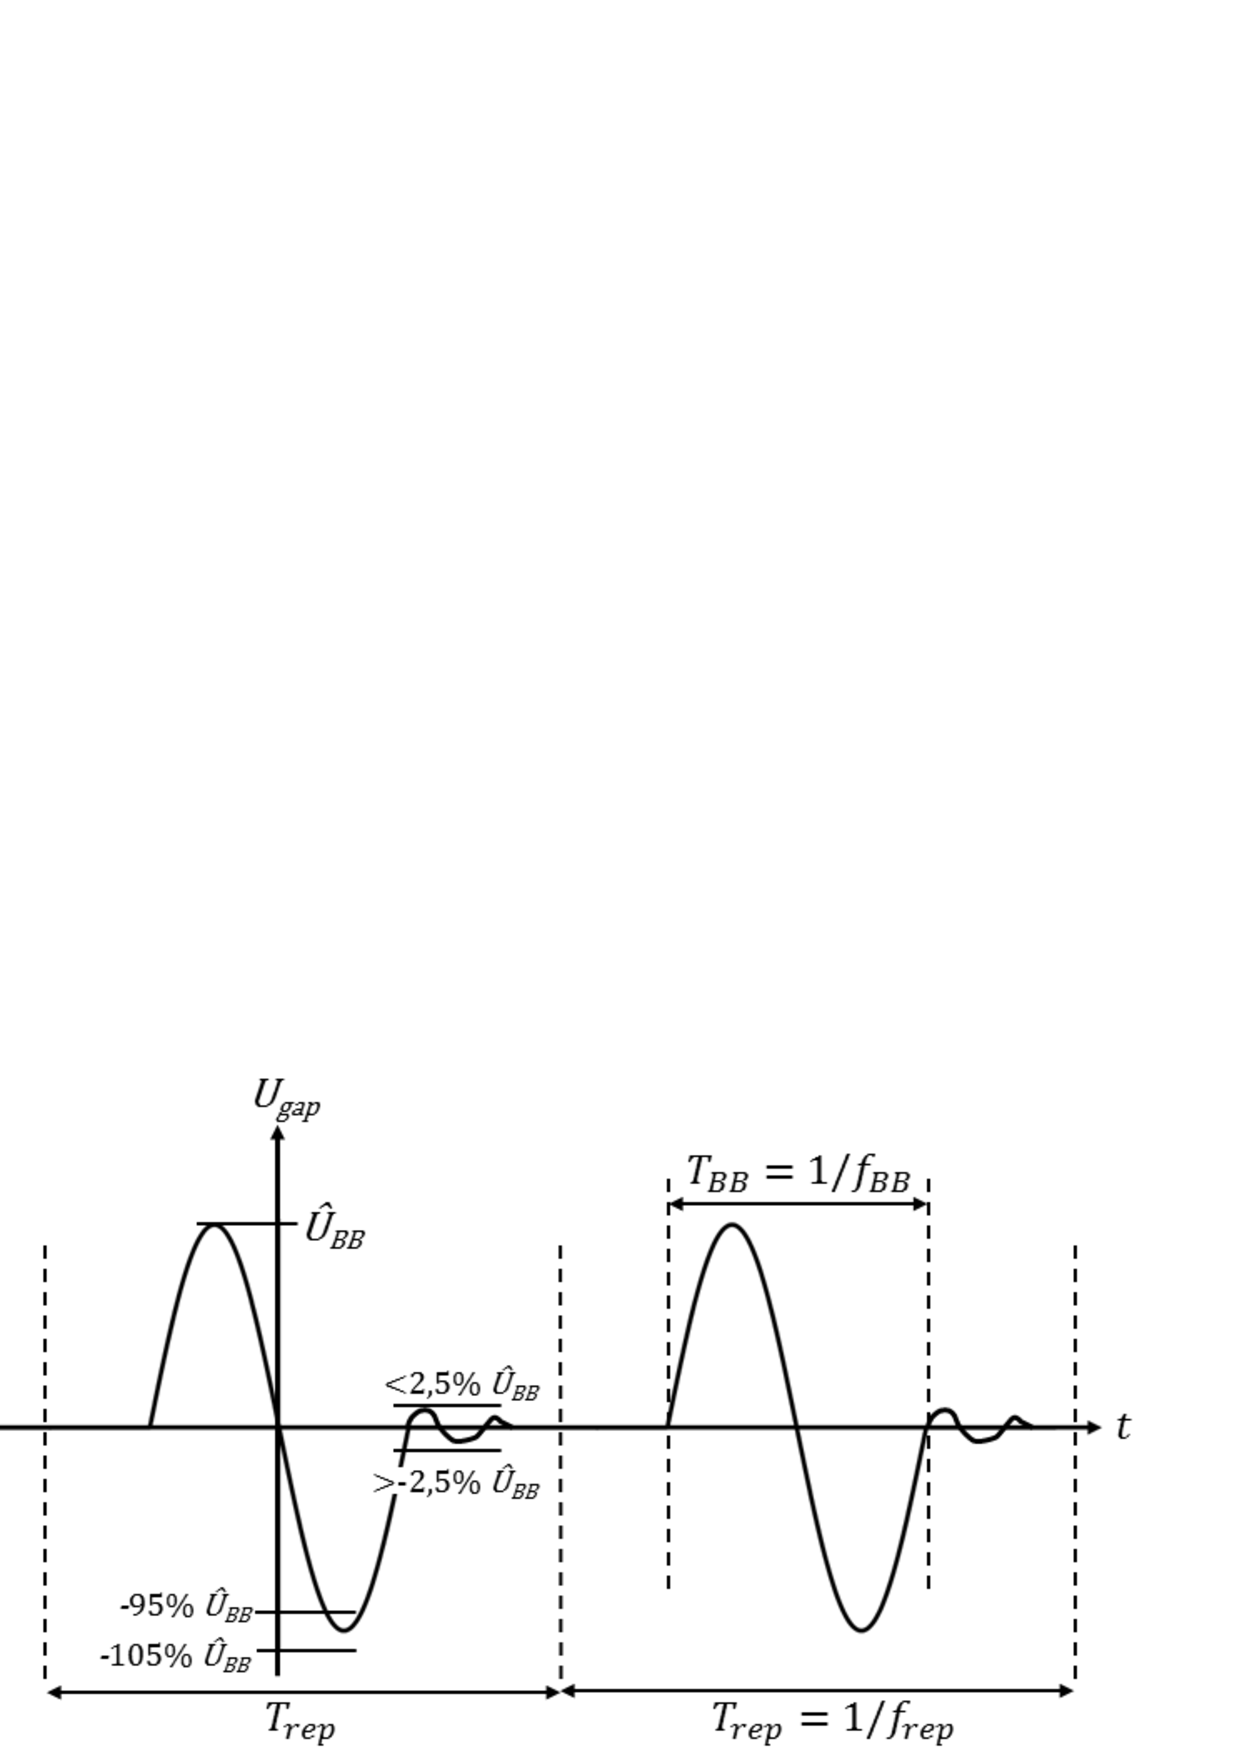
\includegraphics[width=0.5\textwidth]{images/eps/BB_req.pdf}
  \caption{Ausgangssignal}
  \label{fig:BB_req}
\end{figure}
\section[Modell und Konvention]{Modell}
\label{sec:einf.modell_BB}
Der Prototyp des ESR BB besteht aus einem Funktionsgenerator (Keysight 3600A series 2-channel AWG), einem Verstärker (AR1000A225) und der Breitband Ringkern Kavität.\\Dabei kann angenommen werden, dass sich das System bis $\hat{U}_{BB} = 550V$ annähernd linear verhält und durch die Übertragungsfunktion $\underline{H}(\omega)$ beschrieben werden kann. Das
\subsection{ ----- whatever necessary ----}
\label{subsec:einf.modell_BB.name}
--- falls notwendig ---

\section{ --- Motivation PJSem ---- }
\label{sec:einf.motivation}
--- in dieser section wird der Kontext konkretisiert, u. U. auf die Vorarbeit eingegangen --- 
--- je nach Ausführung kann diese section mit der folgenden zusammengelegt werden --- 

\section{ --- Problem / Aufgabenstellung PJSem ---- }
\label{sec:einf.problem}
--- in dieser section wird die konkrete Problemstellung erläutert und damit die Zielsetzung formuliert, 
auf die im Fazit zurückgekommen wird. Das Ziel darf damit auch als \glqq benefit\grqq des Programms im oben beschriebenen Kontext angesehen werden. --- 
\\





\end{document}